\section{Foundation of Our Android App}\label{sec:foundation_of_our_android_app}
This section describes our implementation and adaptation of an example app by Google called \textit{UniversalMusicPlayer}\footnote{\url{https://github.com/googlesamples/android-UniversalMusicPlayer}} as a foundation for our app.
We use this example such that we can focus our project on the device communication and psychoacoustic effects from the beginning, rather than building a generic Android music player with suitable \ac{UI}.
The example is a large codebase, as such we do not cover everything, but rather we present the elements and general implementation choices.
The code provided by Google follows the Android development guidelines, as such this section will introduce the basic Android building blocks that we use in further development of the application.

These basic building blocks of an Android application are: activities and services.

\subsubsection{Activities}\label{subsec:activities}
An \code{Activity} is the primary point of interaction between an application and user.
Each different screen presented to the user is considered a different activity in the application, the media player we use have a fairly limited amount of activities, with \code{MusicPlayerActivity} being the main activity.

The \code{MusicPlayerActivity} holds a instance of \code{MediaController} and \code{MediaBrowser}, which facilitate browsing media and basic playback control features.
All activities in our app uses various views, i.e.~layouts and such. These are \ac{UI} elements and definition, which describes how the app should look.
Most activities inherit from the \code{BaseActivity}, which also includes a \ac{UI} fragment embodying basic playback controls, thereby giving consistency during usage of different activities in the app.
A media player is rarely an application for which an activity is kept active.
An activity has three states, foreground, visible and background.
Having an application run, without its activity visible would be considered a background activity, however these are killable, and by extension so is the process.
For simplicity we will consider leaving an app having no activity in the visible or foreground state.
As such, we need some other way to keep the application alive, such that the application can be allowed to play music, without an activity being either in the state foreground or visible.
To do so we use a service.


\subsubsection{Service}\label{subsec:services}
A service is used to keep an app running in the background for any reason.
They serve to allow apps to perform long-running operations, which happens to be exactly what a media player does.

There are two primary distinctions between services, started services and bound services.
A started service tells the OS to keep it running, even when the user leaves the app.
A bound service is spawned by another app because it wants to utilize the service in some form.
Essentially a bound service is used in order for two processes to communicate, these however are only relevant as long as the application is relevant, as such if the application that caused the service to be spawned is closed, then the service can be killed alongside the application.\cite{androidFundamentals}

In googlesamples we have a started service, \code{MusicService}.
\sloppy\code{MusicService} extends the \code{MediaBrowserServiceCompat} class and implements a playback enabling interface.
It creates a \code{MediaSession}, in doing so it allows the client to create a \code{MediaController} which can send commands to the \code{MediaSession} and thereby perform playback controls without the app having to be actively used.

In \cref{fig:simple_class_diagram}, it is shown how the aforementioned classes belong together.
As previously mentioned, \code{MusicPlayerActivity} inherits from \code{BaseActivity}, which is shown in \cref{fig:simple_class_diagram}.
This is a very simple and minimalistic representation of the app, there are other classes, but these are not relevant in this context.
It is only \code{MusicPlayerActivity}, \code{BaseActivity}, and \code{MusicService} that is shown, since the rest of the mentioned classes are a part of the Android library.

\begin{figure}[!bht]
    \centering
    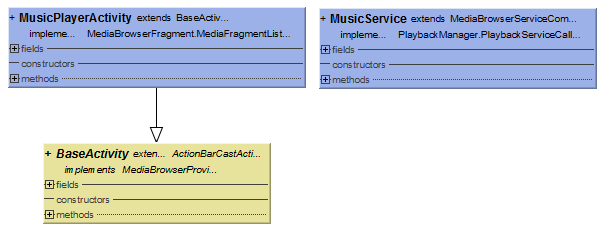
\includegraphics[width=0.8\textwidth]{img/simple_class_diagram.png}
    \caption{A simple diagram of the essential functionality from the example app.}
    \label{fig:simple_class_diagram}
\end{figure}
